%<dscrpt>Fichier de déclarations Latex à inclure au début d'un élément de cours.</dscrpt>

\documentclass[a4paper]{article}
\usepackage[hmargin={1.8cm,1.8cm},vmargin={2.4cm,2.4cm},headheight=13.1pt]{geometry}

%includeheadfoot,scale=1.1,centering,hoffset=-0.5cm,
\usepackage[pdftex]{graphicx,color}
\usepackage[french]{babel}
%\selectlanguage{french}
\addto\captionsfrench{
  \def\contentsname{Plan}
}
\usepackage{fancyhdr}
\usepackage{floatflt}
\usepackage{amsmath}
\usepackage{amssymb}
\usepackage{amsthm}
\usepackage{stmaryrd}
%\usepackage{ucs}
\usepackage[utf8]{inputenc}
%\usepackage[latin1]{inputenc}
\usepackage[T1]{fontenc}


\usepackage{titletoc}
%\contentsmargin{2.55em}
\dottedcontents{section}[2.5em]{}{1.8em}{1pc}
\dottedcontents{subsection}[3.5em]{}{1.2em}{1pc}
\dottedcontents{subsubsection}[5em]{}{1em}{1pc}

\usepackage[pdftex,colorlinks={true},urlcolor={blue},pdfauthor={remy Nicolai},bookmarks={true}]{hyperref}
\usepackage{makeidx}

\usepackage{multicol}
\usepackage{multirow}
\usepackage{wrapfig}
\usepackage{array}
\usepackage{subfig}


%\usepackage{tikz}
%\usetikzlibrary{calc, shapes, backgrounds}
%pour la présentation du pseudo-code
% !!!!!!!!!!!!!!      le package n'est pas présent sur le serveur sous fedora 16 !!!!!!!!!!!!!!!!!!!!!!!!
%\usepackage[french,ruled,vlined]{algorithm2e}

%pr{\'e}sentation du compteur de niveau 2 dans les listes
\makeatletter
\renewcommand{\labelenumii}{\theenumii.}
\renewcommand{\thesection}{\Roman{section}.}
\renewcommand{\thesubsection}{\arabic{subsection}.}
\renewcommand{\thesubsubsection}{\arabic{subsubsection}.}
\makeatother


%dimension des pages, en-t{\^e}te et bas de page
%\pdfpagewidth=20cm
%\pdfpageheight=14cm
%   \setlength{\oddsidemargin}{-2cm}
%   \setlength{\voffset}{-1.5cm}
%   \setlength{\textheight}{12cm}
%   \setlength{\textwidth}{25.2cm}
   \columnsep=1cm
   \columnseprule=0.5pt

%En tete et pied de page
\pagestyle{fancy}
\lhead{MPSI-\'Eléments de cours}
\rhead{\today}
%\rhead{25/11/05}
\lfoot{\tiny{Cette création est mise à disposition selon le Contrat\\ Paternité-Pas d'utilisations commerciale-Partage des Conditions Initiales à l'Identique 2.0 France\\ disponible en ligne http://creativecommons.org/licenses/by-nc-sa/2.0/fr/
} }
\rfoot{\tiny{Rémy Nicolai \jobname}}


\newcommand{\baseurl}{http://back.maquisdoc.net/data/cours\_nicolair/}
\newcommand{\urlexo}{http://back.maquisdoc.net/data/exos_nicolair/}
\newcommand{\urlcours}{https://maquisdoc-math.fra1.digitaloceanspaces.com/}

\newcommand{\N}{\mathbb{N}}
\newcommand{\Z}{\mathbb{Z}}
\newcommand{\C}{\mathbb{C}}
\newcommand{\R}{\mathbb{R}}
\newcommand{\D}{\mathbb{D}}
\newcommand{\K}{\mathbf{K}}
\newcommand{\Q}{\mathbb{Q}}
\newcommand{\F}{\mathbf{F}}
\newcommand{\U}{\mathbb{U}}
\newcommand{\p}{\mathbb{P}}


\newcommand{\card}{\mathop{\mathrm{Card}}}
\newcommand{\Id}{\mathop{\mathrm{Id}}}
\newcommand{\Ker}{\mathop{\mathrm{Ker}}}
\newcommand{\Vect}{\mathop{\mathrm{Vect}}}
\newcommand{\cotg}{\mathop{\mathrm{cotan}}}
\newcommand{\sh}{\mathop{\mathrm{sh}}}
\newcommand{\ch}{\mathop{\mathrm{ch}}}
\newcommand{\argsh}{\mathop{\mathrm{argsh}}}
\newcommand{\argch}{\mathop{\mathrm{argch}}}
\newcommand{\tr}{\mathop{\mathrm{tr}}}
\newcommand{\rg}{\mathop{\mathrm{rg}}}
\newcommand{\rang}{\mathop{\mathrm{rg}}}
\newcommand{\Mat}{\mathop{\mathrm{Mat}}}
\newcommand{\MatB}[2]{\mathop{\mathrm{Mat}}_{\mathcal{#1}}\left( #2\right) }
\newcommand{\MatBB}[3]{\mathop{\mathrm{Mat}}_{\mathcal{#1} \mathcal{#2}}\left( #3\right) }
\renewcommand{\Re}{\mathop{\mathrm{Re}}}
\renewcommand{\Im}{\mathop{\mathrm{Im}}}
\renewcommand{\th}{\mathop{\mathrm{th}}}
\newcommand{\repere}{$(O,\overrightarrow{i},\overrightarrow{j},\overrightarrow{k})$}
\newcommand{\cov}{\mathop{\mathrm{Cov}}}

\newcommand{\absolue}[1]{\left| #1 \right|}
\newcommand{\fonc}[5]{#1 : \begin{cases}#2 \rightarrow #3 \\ #4 \mapsto #5 \end{cases}}
\newcommand{\depar}[2]{\dfrac{\partial #1}{\partial #2}}
\newcommand{\norme}[1]{\left\| #1 \right\|}
\newcommand{\se}{\geq}
\newcommand{\ie}{\leq}
\newcommand{\trans}{\mathstrut^t\!}
\newcommand{\val}{\mathop{\mathrm{val}}}
\newcommand{\grad}{\mathop{\overrightarrow{\mathrm{grad}}}}

\newtheorem*{thm}{Théorème}
\newtheorem{thmn}{Théorème}
\newtheorem*{prop}{Proposition}
\newtheorem{propn}{Proposition}
\newtheorem*{pa}{Présentation axiomatique}
\newtheorem*{propdef}{Proposition - Définition}
\newtheorem*{lem}{Lemme}
\newtheorem{lemn}{Lemme}

\theoremstyle{definition}
\newtheorem*{defi}{Définition}
\newtheorem*{nota}{Notation}
\newtheorem*{exple}{Exemple}
\newtheorem*{exples}{Exemples}


\newenvironment{demo}{\renewcommand{\proofname}{Preuve}\begin{proof}}{\end{proof}}
%\renewcommand{\proofname}{Preuve} doit etre après le begin{document} pour fonctionner

\theoremstyle{remark}
\newtheorem*{rem}{Remarque}
\newtheorem*{rems}{Remarques}

\renewcommand{\indexspace}{}
\renewenvironment{theindex}
  {\section*{Index} %\addcontentsline{toc}{section}{\protect\numberline{0.}{Index}}
   \begin{multicols}{2}
    \begin{itemize}}
  {\end{itemize} \end{multicols}}


%pour annuler les commandes beamer
\renewenvironment{frame}{}{}
\newcommand{\frametitle}[1]{}
\newcommand{\framesubtitle}[1]{}

\newcommand{\debutcours}[2]{
  \chead{#1}
  \begin{center}
     \begin{huge}\textbf{#1}\end{huge}
     \begin{Large}\begin{center}Rédaction incomplète. Version #2\end{center}\end{Large}
  \end{center}
  %\section*{Plan et Index}
  %\begin{frame}  commande beamer
  \tableofcontents
  %\end{frame}   commande beamer
  \printindex
}


\makeindex
\begin{document}
\noindent

\debutcours{Espaces affines}{alpha}

\section{Sous-espaces affines}
\subsection{Direction d'un sous-espace affine}
\begin{defi}
 Soit $E$ un $\K$-espace vectoriel et $\mathcal A$ une partie de $E$. Pour tout élément $\alpha$ de $\mathcal A$, on pose
\begin{displaymath}
 A_\alpha = \left\lbrace a-\alpha, a\in \mathcal A\right\rbrace 
\end{displaymath}
\end{defi}
\begin{defi}
 Soit $E$ un $\K$-espace vectoriel et $A$ une partie de $E$. Pour tout élément $x$ de $E$, on pose
\begin{displaymath}
 x+A = \left\lbrace x+u, u\in \mathcal A\right\rbrace 
\end{displaymath}
\end{defi}
\begin{rem}
 Par définition :
\begin{displaymath}
\mathcal A= a_0 + A_{\alpha}=\left\lbrace  \alpha +x, x\in A_{a_0}\right\rbrace 
\end{displaymath}
\end{rem}

\begin{prop}
 Soit $\mathcal A$ une partie d'un $\K$-espace vectoriel $E$ pour laquelle il existe un $a_0\in\mathcal A$ tel que 
\begin{displaymath}
 A_{a_0} = \left\lbrace a-a_0, a\in \mathcal A\right\rbrace 
\end{displaymath}
est un sous-espace vectoriel de $E$. Alors, pour tout $a_1\in \mathcal A$:
\begin{displaymath}
 A_{a_1} = \left\lbrace a-a_1, a\in \mathcal A\right\rbrace = A_{a_0} 
\end{displaymath}
\end{prop}
\begin{demo}
 On doit prouver deux inclusions.
\begin{itemize}
 \item Montrons que $A_{a_1}\subset A_{a_0}$. Soit $u_1\in A_{a_1}$, il existe $\alpha\in \mathcal{A}$ tel que $u_1=\alpha - a_1$. Alors
\begin{displaymath}
 u_1 = \underset{\in A_{a_0}}{\underbrace{\alpha - a_0}} -\underset{\in A_{a_0}}{\underbrace{(a_1-a_0)}} \in A_{a_0} \hspace{1cm}\text{(stable par addition)}
\end{displaymath}
 \item Montrons que $A_{a_0}\subset A_{a_1}$. Soit $u_0\in A_{a_0}$, il existe $\alpha\in \mathcal{A}$ tel que $u_0=\alpha - a_0$.
\begin{displaymath}
 u_0 = \alpha -a_0 + a_1 -a_1 = 
\underset{\in \mathcal{A}_1}{\underbrace{a_1 + \underset{\in A_1}{\underbrace{(\underset{\in A_1}{\alpha -a_1})-(\underset{\in A_1}{a_0-a_1})}}}} -a_1 \in A_1
\end{displaymath}
\end{itemize}

\end{demo}
\begin{defi}
 On dira qu'une partie $\mathcal A$ d'un $\K$ espace vectoriel $E$ est un sous-espace affine si et seulement si il existe un $a_0\in\mathcal A$ tel que 
\begin{displaymath}
 A_{a_0} = \left\lbrace a-a_0, a\in \mathcal A\right\rbrace 
\end{displaymath}
est un sous-espace vectoriel de $E$. Ce sous-espace vectoriel, indépendant du $a_0$ d'après la pemière proposition est appelé la direction du sous-espace affine.
\end{defi}
\begin{rem}
 Un singleton est un sous-espace affine de direction $\{0_E\}$.
\end{rem}
\begin{defi}
 On dira que deux sous-espaces affines sont parallèles lorsque la direction de l'un est incluse dans la direction de l'autre. 
\end{defi}
\begin{prop}
 Soit $\mathcal A$ un sous-espace affine de direction $A$ et $\mathcal B$ un sous-espace affine de direction $B$. Lorsque $\mathcal A\cap \mathcal B$ est non vide, c'est un sous-espace affine de direction $A\cap B$.
\end{prop}
\begin{demo}
 à rédiger
\end{demo}
\begin{rem}
 Lorsque $A\cap B=\{0_E\}$, l'intersection $\mathcal A \cap \mathcal B$ est soit vide soit réduite à un singleton.
\end{rem}
\begin{prop}
 Soit $\mathcal A$ un sous-espace affine de direction $A$ et $\mathcal B$ un sous-espace affine de direction $B$. Lorsque $A+B=E$, l'intersection $\mathcal A\cap \mathcal B$ est non vide.
\end{prop}
% le fichier de la figure suivante a disparu suite à une ereur de manip
%\begin{figure}[ht]
% \centering
% \input{C5227_1.pdf_t}
% \caption{Projection sur $\mathcal A$ parallélement à B}
% \label{fig:C5227_1}
%\end{figure}

\begin{demo}
 à rédiger
\end{demo}
\begin{prop}
 Soit $\mathcal A$ un sous-espace affine de direction $A$ et $\mathcal B$ un sous-espace affine de direction $B$. Lorsque $A$ et $B$ sont supplémentaires, l'intersection $\mathcal A\cap \mathcal B$ est un singleton.
\end{prop}
\begin{demo}
 à rédiger
\end{demo}
\begin{defi}
 Soit $\mathcal A$ un sous-espace affine de direction $A$, soit $B$ un sous-espace vectoriel supplémentaire de $A$. La projection sur $\mathcal A$ parallélement à $B$ est l'application qui à tout point $m$ de $E$ associe l'unique élément de $\mathcal A \cap(m+B)$.
\end{defi}\index{projection affine}

\subsection{Barycentres}
\begin{prop}[barycentre d'une famille de points pondérés]\index{barycentre d'une famille de points pondérés}
  Soit $(a_1,\cdots,a_p)$ une famille de $p$ points de $E$ et $\alpha_1,\cdots,\alpha_p)$ une famille de $p$ éléments de $\K$ tels que 
\begin{displaymath}
  \alpha_1 + \cdots + \alpha_p \neq 0
\end{displaymath}
Il existe alors un unique $b$ tel que 
\begin{displaymath}
  \alpha_1(b-a_1) + \cdots + \alpha_p(b-a_p) = 0_E 
  \Leftrightarrow b = \frac{\alpha_1}{\sum_{i=1}^p\alpha_i}a_i + \cdots + \frac{\alpha_p}{\sum_{i=1}^p\alpha_i}a_p
\end{displaymath}
Il est applelé barycentre de la famille de points pondéré $((a_i,\alpha_i))_{i\in\llbracket 1,p \rrbracket}$ et noté 
\begin{displaymath}
  \mathcal{B}((a_i,\alpha_i))_{i\in\llbracket 1,p \rrbracket}
\end{displaymath}
\end{prop}

\begin{defi}
 On dira qu'une partie $\mathcal A$ de $E$ est stable par barycentration lorsque, le barycentre d'une famille pondérée (de somme non nulle) quelconque de points de $\mathcal A$ est dans $\mathcal A$.
\end{defi}
\begin{prop}
 Une partie $\mathcal A$ de $E$ est affine si et seulement si elle est stable par barycentration.
\end{prop}
\begin{demo}
Montrons d'abord que su $\mathcal A$ est affine alors elle est stable par barycentration.\newline à rédiger

Montrons maintenant que si $\mathcal{A}$ est stable par barycentration, alors c'est une sous-espace affine.\newline
Soit $a\in \mathcal{A}$ fixé. On doit montrer que $A_a$ est un sous-espace vectoriel.
\begin{itemize}
 \item Soit $x\in A$ et $\lambda \in \K$. Soit $a_x=a+x\in \mathcal A$. Considérons le barycentre $b$ de $\left((a_x,\lambda), (a,1-\lambda) \right)$. Par hypothèse $b\in \mathcal A$ donc $b-a\in A_a$ et 
\begin{displaymath}
 \lambda(a_x-b)+(1-\lambda)(a-b)=0_E
\Rightarrow
\lambda(a_x -a) = b-a
\Rightarrow \lambda x \in A_a
\end{displaymath}
 \item Soit $x$ et $y$ dans $A_a$, notons $a_x=a+x$ et $a_y=a+y$ les deux points de $\mathcal A$ associés. Considérons le milieu $m$ de ces deux points. C'est l'isobarycentre donc il est dans $\mathcal A$. On en tire
\begin{displaymath}
 x+y = 2(m-a)\in A_a
\end{displaymath}
car $m-a\in A_a$ et en utilisant la stabilité par multiplication déjà montrée.
\end{itemize}

\end{demo}
Parties convexes. Une partie est convexe si set seulement si elle est stable par barycentration positive (corps = $\R$).
\subsection{Repères et bases affines}
Repère affine. Fonction coordonnées dans un repère affine. Base affine. Coordonnées barycentriques. Sous-espace affine engendré par une partie. C'est l'intersection de tous les sea contenant cette partie. C'est aussi l'ensemble des barycentres des familles de points de la partie.

\section{Applications affines}
TR\`ES  INCOMPLET: de simples notes ...
\subsection{Définition}
\subsubsection{Partie linéaire}
Définition de $\varphi_a$ par 
\begin{displaymath}
 \forall u\in A : \varphi_a(u)=f(a+u)-f(a)
\end{displaymath}
Proposition-définition : si $\varphi_a$ est linéaire alors tous les $\varphi_b$ sont égaux à $\varphi_a$. On dit alors que $f$ est affine de partie linéaire $\varphi$ (on enlève l'indice dans la notation).
Exemples homothéties, translations.

Dans la suite $f$ est affine de partie linéaire $\varphi$.

\subsubsection{Exemples}
Translations et homothéties, fonctions coordonnées dans un repère, projections affines.

Si $u\in E$ et $f\in \mathcal L(E)$, l'application $m \mapsto u+f(m)$ est affine. Réciproque.
\subsubsection{Barycentres}
\begin{prop}[conservation des barycentres]
 Soit $F$ une appliaction affine de $E$ dans $E$. Pour toute famille de points pondérés $\left((a_1,m_1),\cdots,(a_p,m_p) \right)$ avec $m=m_1+\cdots+m_p\neq0$, le points $F(b)$ est le barycentre de la famille $\left((F(a_1),m_1),\cdots,(F(a_p),m_p) \right)$.  
\end{prop}
\begin{demo}
 à rédiger
\end{demo}
Réciproquement toute application qui conserve la barycentration au sens précédent est  affine.

L'image d'une partie convexes par une application affine est une partie convexe.
\subsection{Opérations}
Espace vectoriel. Composition. Propriété de la fonction partie linéaire. Groupe affine. Une application affine de $E$ dans $E$ est bijective si et seulement si sa partie linéaire est bijective. Groupe des homothéties-translations.

\subsection{Expression en coordonnées}
\subsection{Points fixes}
\index{points fixes d'une application affine}
\begin{prop}
 Soit $F$ une application affine de $E$ dans lui même de partie linéaire $f$. Lorqu'il est non vide, l'ensemble des points fixes pour $F$ est un sous-espace affine de direction $\ker(f-\Id_E)$. 
\end{prop}
\begin{demo}
 à rédiger
\end{demo}
\begin{prop}
 Soit $F$ une application affine de $E$ dans lui même de partie linéaire $f$. Il existe un point fixe pour $F$ si et seulement si il existe $a\in E$ tel que $F(a)-a\in \Im(f-\Id_E)$.
\end{prop}
\begin{demo}
 à rédiger
\end{demo}
\begin{prop}
 Soit $F$ une application affine de $E$ dans lui même de partie linéaire $f$. L'ensemble des points invariants est un singleton si et seulement si $\varphi -\Id_E$ est bijective.
\end{prop}
\begin{demo}
 à rédiger
\end{demo}

\section{Isométries affines d'un plan ou d'un espace}
\subsection{Isométries affines.}
Dans un espace euclidien $E$, la distance entre deux points $a$ et $b$ est la norme de la différence $d(a,b)=\Vert b-a \Vert$.
\index{isométrie}
\begin{defi}
Une isométrie est une application d'un espace euclidien dans lui même qui conserve la distance. 
\end{defi}
\index{question de cours!caractérisation d'une isométrie}
\begin{prop}[caractérisation d'une isométrie]
 Une application d'un espace euclidien dans lui même est une isométrie si et seulement si elle est affine et de partie linéaire orthogonale.
\end{prop}
\begin{demo}Soit $F$ une application d'un espace euclidien $E$ dans lui même. Fixons un $a$ dans $E$ et définissons $f$ 
\begin{displaymath}
 \left\lbrace 
\begin{aligned}
 &E \rightarrow E\\
 &x \mapsto F(a+x) - F(a)
\end{aligned}
\right. 
\end{displaymath}
Supposons que $F$ soit une isométrie. On a donc
\begin{displaymath}
 \forall(u,v)\in E^2,\; \Vert F(u)-F(v)\Vert = \Vert u-v\Vert
\end{displaymath}
Montrons que cela entraine que $f$ conserve le produit scalaire.\newline
Considérons des vecteurs quelconques $x$ et $y$, notons $m=a+x$, $n=a+y$ et écrivons des conservations de distances.
\begin{multline*}
\Vert F(n)-F(m) \Vert ^2 = \Vert F(n)-F(a) +F(a)-F(m) \Vert ^2 \\
= \Vert F(n)-F(a) \Vert ^2 + \Vert F(m)-F(a) \Vert ^2 - 2(F(n)-F(a)/F(m)-F(a)) \\
= \Vert n-a \Vert^2 + \Vert m-a\Vert ^2 - 2(f(x)/f(y))
\end{multline*}
D'autre part
\begin{displaymath}
 \Vert F(n)-F(m) \Vert ^2 = \Vert n-m \Vert ^2 = \Vert n-a \Vert^2 + \Vert m-a\Vert ^2 - 2(x/y) 
\Rightarrow (f(x)/f(y))=(x/y)
\end{displaymath}
Montrons maintenant que $f$ est linéaire.\\
Pour des $x$ et $y$ quelconques dans $E$ et $\lambda$ quelconque dans $\R$:
\begin{multline*}
 \Vert f(x+\lambda y)-f(x)-\lambda f(y)\Vert^2
= \left( f(x+\lambda y)-f(x)-\lambda f(y)/f(x+\lambda y)-f(x)-\lambda f(y) \right)\\
= (f(x+\lambda y)/f(x+\lambda y)) +(f(x)/f(x))+(f(\lambda x)/f(\lambda x)) -2(f(x+\lambda y)/f(x))-2\cdots \\
= (x+\lambda y/x+\lambda y) +(x/x)+(\lambda x/\lambda x) -2(x+\lambda y/x)-2\cdots \text{ (conservation du produit scalaire)}\\ 
= \Vert x+\lambda y-x-\lambda y\Vert^2 = 0 \text{ (bilinéarité du produit scalaire)}
\end{multline*}
La partie linéaire $f$ est alors orthogonale puisqu'elle conserve le produit scalaire.\newline
Réciproquement, si $f$ est linéaire et orthogonale, il est immédiat que $F$ est une isométrie.
\end{demo}
\begin{rem}\index{déplacement}\index{antidéplacement}
Toute isométrie est une bijection affine. On parle d'isométrie directe (déplacement) ou indirecte (antidéplacement) suivant que la partie linéaire est directe ou indirecte. On note $\mathrm{Isom}(E)$, $\mathrm{Isom}^+(E)$ et $\mathrm{Isom}^-(E)$ les ensembles correspondants. Il est immédiat que les isométries forment un sous-groupe du groupe des bijections de $E$ et que les déplacements forment un sous-groupe du groupe des isométries. 
\end{rem}
\index{rotation affine}
\begin{defi}[rotation affine]
 Soit $E$ euclidien de dimension $2$ ou $3$. Une \emph{rotation affine} est une application de la forme
\begin{displaymath}
 \left\lbrace 
\begin{aligned}
 &E \rightarrow E \\
 &m \mapsto a+f(m-a)
\end{aligned}
\right. 
\end{displaymath}
où $a\in E$ et $f\in \mathcal O^+(E)$.
\end{defi}
\begin{rems}
\begin{enumerate}
 \item L'ensemble des points fixes d'une rotation ainsi définie est 
\begin{itemize}
 \item la droite affine $a+\Vect(w)$ où $w$ est un vecteur directeur de l'axe de $d$ dans le cas de la dimension $3$.
 \item le singleton $\{a\}$ dans le cas de la dimension $2$. 
\end{itemize}
\item Une rotation est un déplacement
\end{enumerate}
\end{rems}

\index{symétrie affine}
 \begin{defi}[symétrie affine]
 Soit $E$ euclidien de dimension $2$ ou $3$. Une \emph{symétrie affine} est une application de la forme
\begin{displaymath}
 \left\lbrace 
\begin{aligned}
 &E \rightarrow E \\
 &m \mapsto a+f(m-a)
\end{aligned}
\right. 
\end{displaymath}
où $a\in E$ et $f$ est une symétrie orthogonale.
\end{defi}
\begin{rems}
 \begin{enumerate}
  \item On parle de réflexion affine ou de retournement affine suivant le type de la partie linéaire. Une réflexion affine est un antidéplacement. En dimension $3$, un retournement est un déplacement.
  \item Lorsque la partie linéaire est une symétrie par rapport à un sous-espace vectoriel $V$, l'ensemble des points fixes de la symétrie affine est le sous-espace affine passant par $a$ et de direction $V$. On parle alors de symétrie par rapport à un sous-espace affine.
 \end{enumerate}
\end{rems}


\index{symétrie glissée}
\begin{defi}[symétrie glissée]
Une \emph{symétrie glissée} est la composée d'une symétrie affine et d'une translation dont le vecteur est dans la direction du sous-espace par rapport auquel se fait la symétrie. 
\end{defi}
\begin{figure}[h!t]
 \centering
 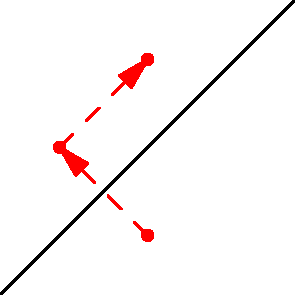
\includegraphics{C5727_1.pdf}
 % C5727_1.pdf: 0x0 pixel, 0dpi, nanxnan cm, bb=
 \caption{symétrie glissée en dimension $2$}
 \label{fig:C5727_1}
\end{figure}


\index{vissage}
\begin{defi}[vissage]
 Pour un espace de dimension $3$. Un \emph{vissage} est la composée d'une rotation affine et d'une translation dont le vecteur est dans la direction de l'axe de la rotation. 
\end{defi}
\begin{figure}[ht!]
 \centering
 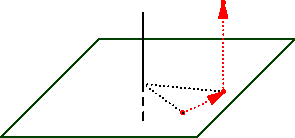
\includegraphics{C5727_2.pdf}
 % C5727_2.eps: 0x0 pixel, 0dpi, 0.00x0.00 cm, bb=
 \caption{vissage en dimension $3$}
 \label{fig:C5727_2}
\end{figure}

\index{rotation-miroir affine}
\begin{defi}[rotation-miroir affine]
 Pour un espace de dimension $3$. Une \emph{rotation-miroir} est la composée d'une rotation affine et d'une réflexion affine par rapport à un plan orthogonal à l'axe de la rotation. 
\end{defi}




Exemple symétries affines.
\subsection{Classification.}
Définition d'une symétrie par rapport à une droite affine. Définition d'une rotation affine. ( avec point fixe + partie linéaire). Définition d'une symétrie glissée.  
\index{question de cours!classification des isométries!plan}
Classification Toute isométrie affine est soit une translation, soit une rotation, soit une réflexion-glissée.
\subsubsection{Dans un plan.}
\index{question de cours!classification des isométries!espace}
\subsubsection{Dans un espace.}
Définition d'une rotation autour d'un axe (avec pt fixe + partie linéaire) d'un vissage, d'une réflexion glissée, d'une rotation-miroir affine. \index{réflexion glissée}

Classification. Toute isométrie affine est soit un vissage (déplacement) soit une réflexion-glissée soit une rotation-miroir (antidéplacements).
\subsection{Similitudes directes d'un plan}
\end{document}
